\begin{frame}
\frametitle{Clasificación de problemas}

Primera clasificación:

\begin{itemize}
\item \textit{Entscheidungsproblem} (El problema de decisión).
\pause
\begin{columns}
\column{0.5\textwidth}
\begin{figure}

\includegraphics[scale=0.096]{./images/Turing.jpg}
\caption{Alan Turing}
\end{figure}
\column{0.5\textwidth}
\begin{figure}
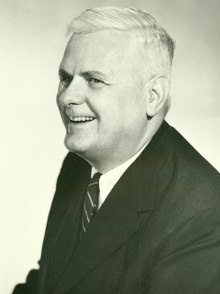
\includegraphics[scale=0.3]{./images/Church.jpg}
\caption{Alonzo Church}
\end{figure}
\end{columns}
\pause
\item Medición de tiempo y espacio en función de la entrada.
\begin{itemize}
\item Juris Hartmanis.
\item Richard Stearns.
\end{itemize}
\end{itemize}
\end{frame}



\begin{frame}
\frametitle{Clasificación de problemas}
Clases de complejidad:
\begin{itemize}
\item El lenguaje $L$ está en \textsl{P} $\Leftrightarrow$ cumple que: 
\begin{itemize}
\item $M$ corre en tiempo polinomial para toda entrada
\item $\forall x \in L, M(x) = TRUE \lor FALSE$.
\end{itemize}
\pause
\item Un lenguaje $L \in $ \textsl{NP} $\rightarrow \exists$ un
  polinomio $p: \mathbb{N} \longrightarrow \mathbb{N}$ y una MT $M$ 
  tal que $\forall x \in \{0,1\}^{*}$, 
  
  \begin{displaymath}
    x \in L \Leftrightarrow \exists u \in \{0,1\}^{p(|x|)},~
    \textrm{tal que} ~ M(x,u) = 1.
  \end{displaymath}
  \pause
\item Se dice que $L'$ es \textsl{NP}-duro si
  $L \leq_{p} L'$ para cada $L \in \textsl{NP} $.
  \pause
\item  Se dice que $L'$ es \textsl{NP}-completo si $L'$ es \textsl{NP}-duro y
  $L' \in \textsl{NP}$.
\end{itemize}

%\begin{itemize}
%\item Ejemplo de \textsl{NP}-completo: \texttt{3-PARTITION}
%\end{itemize}
\end{frame}